\documentclass[tikz]{standalone}
\usetikzlibrary{positioning}

\begin{document}
	
	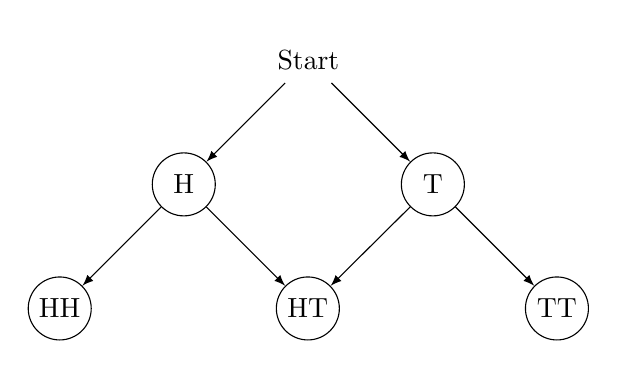
\begin{tikzpicture}[
		every node/.style={circle, draw, minimum size=8mm, inner sep=0pt},
		edge from parent/.style={draw, -latex},
		level distance=1.5cm,
		sibling distance=3cm
		]
		
		% Root node
		\node[draw=none] (start) {Start};
		
		% First level
		\node[below left=of start] (H1) {H};
		\node[below right=of start] (T1) {T};
		
		% Second level
		\node[below left=of H1] (HH) {HH};
		\node[below right=of H1] (HT) {HT};
		\node[below right=of T1] (TT) {TT};
		
		% Connect edges
		\draw[-latex] (start) -- (H1);
		\draw[-latex] (start) -- (T1);
		
		\draw[-latex] (H1) -- (HH);
		\draw[-latex] (H1) -- (HT);
		
		\draw[-latex] (T1) -- (HT);
		\draw[-latex] (T1) -- (TT);
		
	\end{tikzpicture}
	
\end{document}

